\begin{figure}[t]
\centering
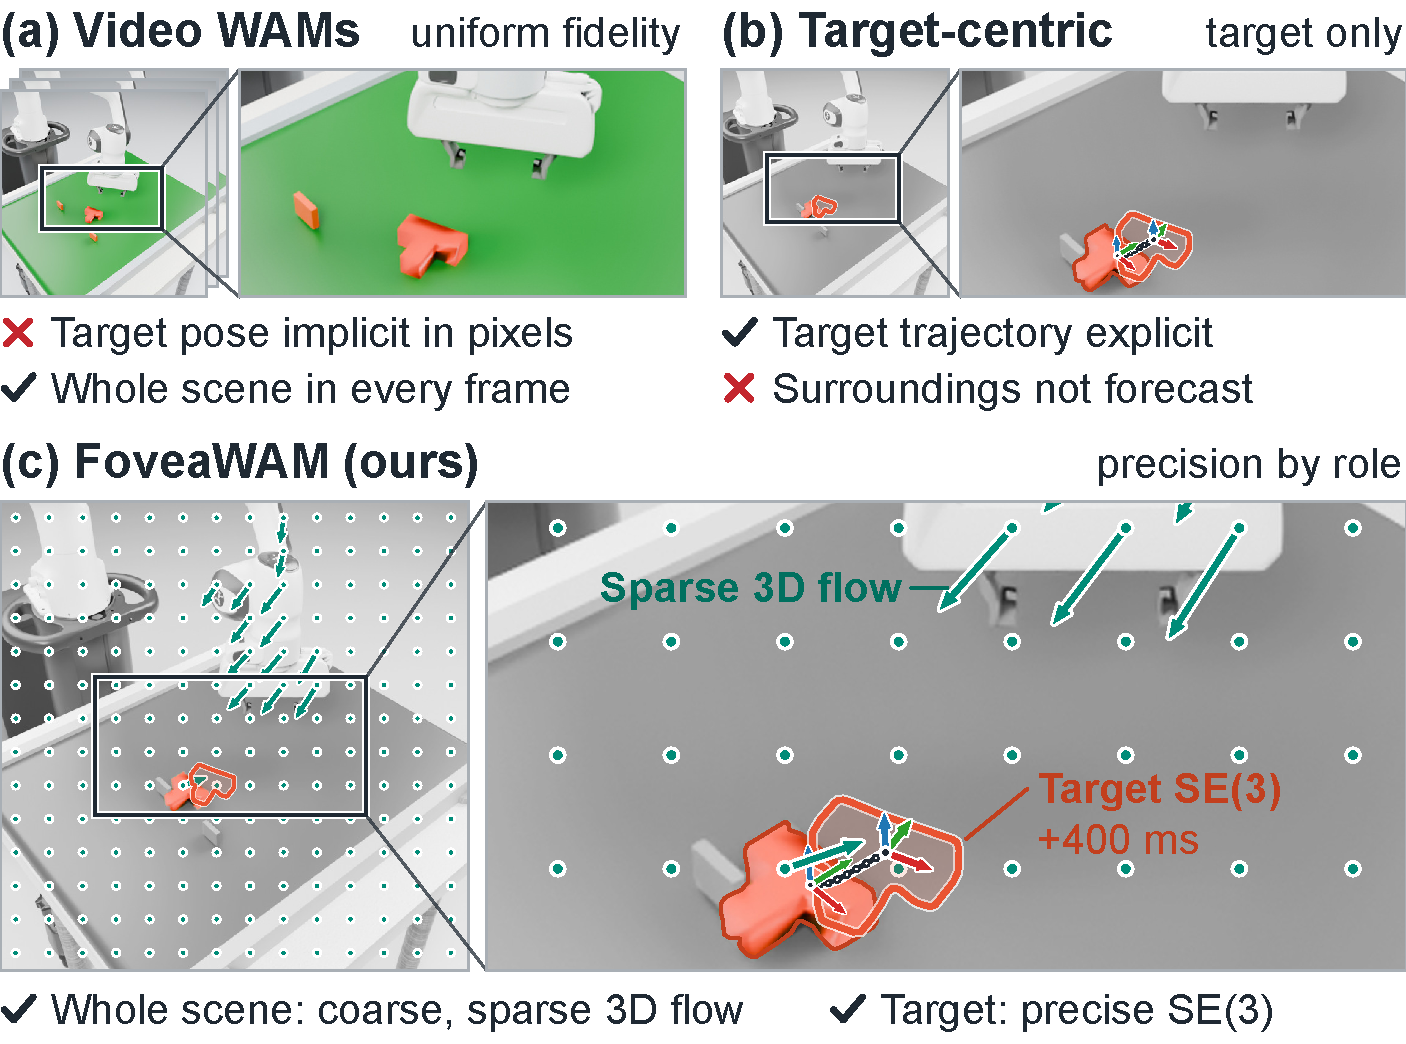
\includegraphics[width=\columnwidth]{figures/paradigms/paradigms.pdf}
\caption{\textbf{Where forecast precision goes.}
Three forecast representations illustrated with one recorded \bench scene (agent view; boxed region enlarged).
(a) Video WAMs forecast frames or latents at uniform fidelity; the target's metric pose stays implicit \cite{dreamzero,openwam_alpha}.
(b) Target-centric predictors forecast only the target's trajectory \cite{domino,spot}.
(c) From one RGB-D frame and the target's SE(3) history, \ours forecasts the whole scene coarsely as sparse 3D flow on a \cfgContextGrid{} grid (teal; dots: displacement $\leq 2$\,mm), where one sample lands on the target, and the target's SE(3) trajectory precisely (orange; axes: pose now and at $+400$\,ms). Both forecasts supervise training and are skipped at inference. Overlays come from the recording.}
\label{fig:paradigms}
\end{figure}
